\documentclass[11pt]{article}
\usepackage[letterpaper,margin=1in]{geometry}
\usepackage{mytex}
\usepackage[colorlinks=true,linkcolor=blue,citecolor=blue]{hyperref}%

\usepackage{bookmark}

\usepackage{newtxtext, kotex}
\usepackage[all,cmtip]{xy}
\usepackage{tikz}
\usepackage{pgfplots}
\usepackage{caption}


\usepackage{fancyhdr}
%\fancyhf{} % sets both header and footer to nothing
\renewcommand{\headrulewidth}{0pt}


\usepackage[textwidth=1in,textsize=small,colorinlistoftodos]{todonotes} % todo 노트

\pagestyle{fancy}
\lhead{Myungsin Cho}
\chead{}
\rhead{\univ \\ Ph.D. Mathematics}
%\rfoot{\date}

%Bibliography line spacing
% ADD THE FOLLOWING COUPLE LINES INTO YOUR PREAMBLE
\let\OLDthebibliography\thebibliography
\renewcommand\thebibliography[1]{
  \OLDthebibliography{#1}
  \setlength{\parskip}{0pt}
  \setlength{\itemsep}{0pt plus 0.3ex}
}

% section 폰트 바꿔주는거
\usepackage{titlesec}
\titleformat{\section}{\normalfont\large\center}{\thesection}{.5em}{}
\titleformat{\subsection}[runin]{\normalfont\bfseries}{\thesubsection}{.5em}{}

\newcommand{\yourname}{Myungsin Cho}

\newcommand{\univ}{Indiana University}

\newcommand\quelle[1]{{%
      \unskip\nobreak\hfil\penalty50
      \hskip2em\hbox{}\nobreak\hfil #1%
      \parfillskip=0pt \finalhyphendemerits=0 \par}}
      

\usepackage{amsmath,amsfonts,amssymb,mathrsfs}
\usepackage{amsthm,thmtools}
\newtheorem{theorem}{Theorem}
\newtheorem{proposition}{Proposition}
\newtheorem{lemma}{Lemma}
\newtheorem{corollary}[theorem]{Corollary}
\newtheorem*{goal}{Goal}

\let\overto\xrightarrow

\begin{document}
\begin{center}\LARGE{Research Statement}
\end{center}

Algebraic topology originated as a field employing algebraic methods to analyze and classify spaces.  As the field has developed over time, it has come to play a central role in the interaction between algebra and topology in modern mathematics.
My research investigates how tools from algebraic topology can illuminate the properties of complex algebraic systems, including number fields or commutative rings with group action.
This can be done by exploring the connections at the intersection of stable homotopy theory with algebraic K-theory, equivariant algebra, and combinatorics, often revealing insights relevant to number theory and arithmetic geometry.
I aim to advance our understanding of algebraic invariants and equivariant objects across these interconnected fields by developing new methods and uncovering precise correspondences between different mathematical descriptions.

\section{Current research and direction}

My current research program is centered around several interconnected projects that explore fundamental structures and relationships in {\it stable homotopy theory}, {\it algebraic K-theory}, and {\it equivariant algebra}, often drawing connections to number theory and combinatorics.

In topology, K-theory is the study of vector bundles over topological spaces which can be thought of as a family of vector spaces parameterized by points of a space, varying continuously.
Simple examples include the Mobius band (a non-trivial bundle) and the cylinder (a trivial bundle) which serve as basic illustrations of different types of vector bundles over a circle:
\vspace{-1.5em} 
\begin{center}
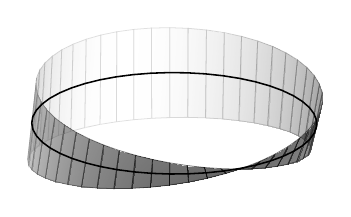
\begin{tikzpicture}[scale=0.7]
\begin{axis}[
    hide axis,
    zmin=-1, zmax=1,
    view={70}{30}
]
\addplot3 [
    surf, shader=faceted interp,
    opacity=0.6,
    point meta=x,
    colormap = {whiteblack}{color(0cm)  = (white);color(1cm) = (black)},
    samples=50,
    samples y=2,
    z buffer=sort,
    domain=0:360,
    y domain=-0.5:0.5
] (
    {(1+0.1*y*cos(x/2))*cos(x)},
    {(1+0.1*y*cos(x/2))*sin(x)},
    {1*y*sin(x/2)});

\addplot3 [
    samples=50,
    domain=-110:250, % The domain needs to be adjusted manually, depending on the camera angle, unfortunately
    samples y=0,
    thick
] (
    {cos(x)},
    {sin(x)},
    {0});
\end{axis}
\end{tikzpicture}
\hspace{2em}
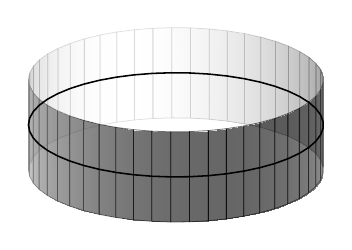
\begin{tikzpicture}[scale=0.7]
\begin{axis}[
    hide axis,
    zmin=-1, zmax=1,
    view={70}{30}
]
\addplot3 [
    surf, shader=faceted interp,
    opacity=0.6,
    point meta=x,
    colormap = {whiteblack}{color(0cm)  = (white);color(1cm) = (black)},
    samples=50,
    samples y=2,
    z buffer=sort,
    domain=0:360,
    y domain=-0.5:0.5
] (
    {cos(x)},
    {sin(x)},
    {y});

\addplot3 [
    samples=50,
    domain=-110:250, % The domain needs to be adjusted manually, depending on the camera angle, unfortunately
    samples y=0,
    thick
] (
    {cos(x)},
    {sin(x)},
    {0});
\end{axis}
\end{tikzpicture}
\\[-1em] % reduce vertical space
\parbox{6cm}{\centering \small Mobius band over a circle}
\hspace{0em}
\parbox{6cm}{\centering \small Cylinder over a circle}
\end{center}

Interestingly, this way of studying bundles gives rise to a subtle invariant of spaces and appears in many branches of mathematics, such as number theory, algebraic geometry, geometric topology, and differential topology.

\subsection{Algebraic K-theory and Arithmetic Duality}
My dissertation work explores deep connections between algebraic K-theory, number theory, and topology, focusing on fundamental questions about the structure of rings of integers in number fields and related objects. {\it Algebraic K-theory} is a powerful invariant that captures both algebraic and geometric information, playing a central role in arithmetic geometry. A fundamental duality this area is {\it arithmetic Tate-Poitou duality}, which describes profound relationships between the cohomology groups of number rings and their completions. Motivated by the intricate relationships described by fundamental arithmetic dualities like Tate-Poitou duality, exploring their K-theoretic analogues has become an important direction of investigation.

My work \cite{Cho} establishes a crucial step towards this goal by proving {\it K-theoretic Tate-Poitou duality at prime 2}. This theorem provides a homotopical refinement of the classical arithmetic duality, revealing structural relationships within the {\it $K(1)$-localized algebraic K-theory} of a number ring and its completions. Specifically, for a number field $F$, I prove a {\it canonical weak equivalence} between the {\it homotopy fiber of the completion map} $\ka$ in $K(1)$-local algebraic K-theory:
\[\ka: L_{K(1)}K(\calO[\tfrac{1}{2}]) \to \prod_{\nu\in S} L_{K(1)}K (F_\nu^\w)\]
 and a form of {\it $\bZ_2$-Anderson dual} applied to the algebraic K-theory of the input ring: 
\[\Fib(\ka) \simeq \SI^{-1} I_{\bZ_2} L_{K(1)}K(\calO_F[\tfrac{1}{2}]).\]

A significant application and consequence of this main duality theorem is a new insight into the algebraic K-theory of the {\it sphere spectrum} ($\bS$). The sphere spectrum, a fundamental object in stable homotopy theory, behaves in many ways like a ring of integers in classical algebra. Using my K-theoretic Tate-Poitou duality (specifically, for the rational numbers $\bQ$), combined with foundational results in the field, I proved that the connective cover of the homotopy fiber of the 2-completed {\it cyclotomic trace map} $\ta_\bS$ for the sphere spectrum:
\[\ta_\bS: K(\bS)_2^\w \to TC(\bS)_2^\w\]
 is weakly equivalent to the $\bZ_2$-Anderson dual of the $K(1)$-localized algebraic K-theory of the integer: 
\[\Fib(\ta_\bS)[0,\infty) \simeq \SI^{-1}I_{\bZ_2} L_{K(1)} K(\bZ)[0,\infty).\] This result provides a powerful computational handle on the algebraic K-theory of $\bS$ at prime 2 and highlights a deep connection between stable homotopy theory and the arithmetic of the integers via algebraic K-theory.
Furthermore, the homotopy fiber of the completion map $\Fib(\ka)$ that appears in K-theoretic Tate-Poitou duality is known to be related to objects studied in other areas, including the {\it $p$-adic Langlands correspondence} \cite{MR2905536} and {\it compactly supported K-theory} \cite{MR3211458}. My work, by providing a rigorous description of this fiber at prime 2, offers potential avenues for exploring these connections.

This work extends foundational results by Blumberg, Mandell and Yuan \cite{MR4121155,BMY}, who proved this duality for odd primes and conjectured its validity for the prime 2 case. The prime 2 case presents unique and significant challenges due to the essential role of real embeddings of the number field, which fundamentally alters the behavior of related invariants and necessitates new technical machinery not required in the odd prime setting.

This research provides crucial new results and techniques in algebraic K-theory, offering significant insights into the structure of algebraic K-theory for number rings and providing powerful tools for computations related to fundamental objects like the sphere spectrum. The K-theoretic Tate-Poitou duality established here has numerous potential implications and suggests several directions for future investigation in more general settings.

\subsection{Real Algebraic K-theory}
Another ongoing project focuses on {\it real algebraic K-theory} and its computational methods. In collaboration with Teena Gerhardt, Liam Keenan, Juan Moreno, and J.D. Quigley, our research contributes to this area by extending {\it homological trace methods} due to Bruner and Rognes \cite{MR2153113} to the $C_2$-equivariant setting. This work develops a new spectral sequence approach, rooted in using $RO(C_2)$-graded homology, designed to provide computational access to invariants in real algebraic K-theory. This approach enhances classical trace methods to the real setting, aiding in the understanding and approximation of real algebraic K-theory for key objects like the {\it real bordism spectrum} ($MU_\bR$).
 
Real algebraic K-theory arises when a ring is equipped with an {\it anti-involution}—a type of symmetry operation—and we seek algebraic invariants that respect this structure. As introduced by Hesselholt and Madsen \cite{HMreal}, real algebraic K-theory provides such an invariant: it is a genuine $C_2$-equivariant spectrum that naturally unifies and extends classical algebraic K-theory, Hermitian K-theory, and L-theory by taking into account the ring's anti-involution. Understanding real algebraic K-theory is crucial for gaining insights into the structure of rings with anti-involution and their connections to topology and geometry.
Recent advancements in real algebraic K-theory have largely stemmed from the development of {\it real trace methods}, powerful computational techniques rooted in equivariant stable homotopy theory. These methods have produced real analogues of classical results and tools, including the construction of {\it real topological Hochschild homology} \cite{Dotto} and {\it real topological cyclic homology} \cite{Hogenhaven}. Our specific extension of homological trace methods builds upon this progress.

An ultimate goal of this collaborative work is to utilize these new real homological trace methods to better understand and approximate the real algebraic K-theory of important objects like the {\it real bordism spectrum} ($MU_\bR$) and {\it real Brown-Peterson spectrum} ($BP_\bR$). Our approach aims to establish a {\it real analogue of the Segal conjecture} for such spectra, which serves as a crucial tool in this approximation. Achieving such an analogue would provide essential computational tools and deepen our understanding of the relationship between real algebraic K-theory and its trace method approximations.


\subsection{Equivariant algebras and homotopical combinatorics}
My research in {\it equivariant algebra} investigates the correspondence between combinatorics and the algebra underlying equivariant stable homotopy theory. At its heart are {\it transfer systems} \cite{MR4244201}, which are fascinating combinatorial objects defined on the subgroup lattice of a group $G$. A transfer system is essentially a way of selecting a subset of possible ``transfer'' operations between subgroups, specified by a partial order on the subgroups that refines the usual inclusion, and is consistent with conjugation and restriction to smaller subgroups. These discrete combinatorial structures play a surprising and fundamental role in describing $G$-equivariant algebraic objects in stable homotopy theory.

Specifically, the algebraic structures capturing the homotopy groups of {\it commutative $G$-ring spectra} are known as {\it Tambara functors} \cite{MR1209937} and their variations, like {\it incomplete} or {\it bi-incomplete} Tambara functors\cite{MR3773736,MR4327103}. The structure of these functors, particularly the presence or absence of certain additive (transfers) and multiplicative operations (norms), is precisely encoded by the data of one or more associated transfer systems which satisfies specific coherence conditions \cite{MR4696086}. Thus, understanding transfer systems is crucial for understanding the $N_\infty$-operadic algebra structure underlying equivariant stable homotopy theory.

In collaboration with David Chan, David Mehrle, Pablo Sanchez Ocal, Angelica Osorno, Ben Szczesny, and Paula Verdugo, our work establishes a fundamental equivalence between two descriptions of the structures governing incomplete Tambara functors. One is a combinatorial description using compatible pairs of transfer systems. The other is an homotopical description using {\it actions of operads} \cite{MR2544392}. Our team has proved one direction of this equivalence: that an action of one $N_\infty$-operad on another implies their associated transfer systems form a compatible pair. A primary goal of our ongoing work is to prove the converse – that a compatible pair of transfer systems can be realized as $N_\infty$-operad action. Proving this equivalence is significant because it provides a unified understanding of the structures governing incomplete Tambara functors by bridging combinatorial and operadic perspectives. 


\section{Future research direction}
My future research directions build upon the foundations laid by my current work, naturally extending established results and exploring related open questions in algebraic K-theory, equivariant algebra, and their connections to other fields. Beyond these direct continuations, I am also dedicated to identifying research topics that are accessible, particularly to undergraduate students. Creating opportunities for students to learn about these exciting areas and make meaningful contributions is important to me, as I believe it fosters the next generation of researchers in algebraic topology and related fields.

\subsection*{Duality and Symmetry in Algebraic K-theory}
Building upon my established work on K-theoretic Tate-Poitou duality, several avenues for future research emerge, exploring analogues in broader mathematical settings and developing related areas of algebraic K-theory.

One natural direction is to investigate the higher-dimensional counterparts of K-theoretic duality.  Recent progress has been made in this area for odd primes \cite{Braunling}, and my expertise in handling the unique challenges at the prime 2 positions me to extend these higher-dimensional results to include this case.

Another promising direction lies in exploring this duality for higher chromatic height in stable homotopy theory. Initial results \cite{HRW} suggest that certain objects behave in ways analogous to classical local rings, and my goal is to establish K-theoretic Tate-Poitou duality for these types of localized structures.

Beyond extending duality, I am also focused on real algebraic K-theory. This area presents many open questions, particularly in adapting classical algebraic K-theory concepts and results to this setting with symmetry.


\subsection*{Foundations for Equivariant Algebra}
While advanced structures like Tambara functors are powerful tools in equivariant stable homotopy theory, many fundamental algebraic concepts that are standard for classical rings remain  underdeveloped or missing in this setting. 

This project is approachable at different levels. Even in the case of $G$-rings (a simpler type of equivariant algebraic object that Tambara functors generalize), many elementary definitions and properties are still unclear. For example, defining algebraic extensions and algebraic closures for $G$-rings presents interesting challenges. Working on these questions for $G$-rings is a concrete starting point that is accessible even to undergraduate students and provides valuable insight before tackling the more complex general Tambara functor case. By starting with these more manageable, we can build intuition and techniques applicable to the broader theory of Tambara functors.

My goal is to establish these fundamental algebraic concepts and structures within this equivariant setting. This foundational work is crucial for eventually developing an algebraic geometry of Tambara functors.

\subsection*{Transfer Systems and Homotopical Combinatorics}
Another exciting direction for future research lies in exploring {\it transfer systems} from a purely combinatorial perspective. While deeply connected to equivariant stable homotopy theory, transfer systems have a remarkably elementary definition based on the subgroup lattice of a group. This discrete, combinatorial nature makes them highly accessible, even to undergraduate students who may not have extensive background in advanced topology or algebra. Simple combinatorial questions about these structures, such as counting problems for finite posets derived from transfer systems, can lead to surprising and non-trivial insights into stable homotopy theory. 

This interplay between combinatorics and homotopy theory is a growing area, sometimes referred to as {\it homotopical combinatorics}, and it has proven fruitful for undergraduate research projects, demonstrating its accessibility and potential for discovery. Continuing to explore the combinatorial properties of transfer systems offers a promising path for both foundational understanding and engaging new researchers.

\subsection*{Topological data analysis}
An exciting and rapidly emerging area is {\it Topological Data Analysis} (TDA), which uses tools from algebraic topology to find ``shape'' within complex datasets. TDA provides methods to detect underlying shape of data, offering a unique perspective that complements traditional techniques.

This area is increasingly revealing deep connections with advanced mathematical fields, including algebraic K-theory and equivariant homotopy theory. These connections are a focus of current research, exploring how powerful invariants from these fields can provide new theoretical frameworks and computational tools to better understand the structure and complexity of the topological spaces derived from data. The growing importance of this intersection is highlighted by events like the upcoming conference on Homotopy Theory and Topological Data Analysis at the Fields Institute \href{http://www.fields.utoronto.ca/activities/25-26/homotopy-theory}{(link)}, which specifically explores these links between theoretical topology and real-world data challenges.

TDA is particularly promising for students, including undergraduates, due to its intuitive ideas and visual nature. Techniques like {\it persistent homology} can be explained by thinking about data points as a cloud and observing how topological features appear and disappear across scales. This allows students to apply sophisticated math to tangible problems, demonstrating the power of abstract mathematics in practical applications and providing a pathway for research contributions.

\subsection*{Analytic Stacks and Hyperbolicity}
Another area of future research involves using advanced mathematical language to study complex geometry, specifically focusing on hyperbolicity.
Working with my collaborator, Geonhee Cho, we are interested in extending the concepts of hyperbolicity to more general types of geometric objects known as analytic stacks or groupoids. Defining and understanding hyperbolicity for these more intricate structures is a key goal.

Our collaboration aims to investigate how hyperbolicity conditions on these analytic stacks interact with their underlying geometric properties. We are eager to explore how being hyperbolic might imply rigidity phenomena or place asymptotic constraints on these complex spaces. This work has the potential to uncover new insights into the structures of  automorphisms, how curvature behaves, and phenomena related to symmetry breaking in these generalized geometric settings.

\section{Conclusion}
In summary, my research explores the deep connections between stable homotopy theory, algebraic K-theory, equivariant algebra, and combinatorics. Building on my work establishing K-theoretic duality at prime 2 and investigating equivariant algebraic structures, my future directions aim to extend these dualities to more general setting, develop foundational algebraic concepts for Tambara functors, and explore connections to analytic stacks and hyperbolicity. Crucially, my research also includes projects on transfer systems and topological data analysis, which offer accessible entry points for undergraduate students to contribute to cutting-edge mathematics, fostering the next generation of algebraic topologists.

\bibliography{RS_bib}
\bibliographystyle{alphaurl}

\end{document}